%% Latex Template for MSc projects - Deliverable I
%% School of Science, Computer Science Department
%% Loughborough University
%% Prepared by Andrea Soltoggio, 2018

\documentclass[12pt,oneside,a4paper]{article}
\usepackage[utf8]{inputenc}
\usepackage[english]{babel}
\usepackage{fancyhdr}
\usepackage{graphicx}
\usepackage{cite}
\usepackage[hyphens]{url}
\usepackage[hidelinks]{hyperref}
\hypersetup{breaklinks=true}
\urlstyle{same}
\usepackage{booktabs}

\usepackage{CJK}

%chapter


%\setlength{\arrayrulewidth}{1mm}
\setlength{\tabcolsep}{6pt}
\renewcommand{\arraystretch}{1.5}

\renewcommand{\baselinestretch}{1.15}

%----------------------------------------------------------------------------------------
%	TITLE PAGE
%----------------------------------------------------------------------------------------

% Create the command for including the title page with \makeTatlePage command



\newcommand*{\maketitledavid}{
    \thispagestyle{empty}
    \begin{center}
    	\vspace*{2cm}
    	
\includegraphics[width = 7cm]{images/LoughboroughLogo.png} \par
    	\vspace{2cm}
    	\textbf{\LARGE{\fontsize{12pt}{50pt}AI Assisted Bone Fracture Detection and Localization from Multi-view X-Ray Images}} \par
    	\vspace{1cm}
    	\textbf{\normalsize{Weipeng Wu}} \par
	\textbf{\normalsize{B836051}} \par
	\textbf{\normalsize{Superviser: Dr. Lianghao Han}} \par

    	\vfill 
	\textbf{\small {MSc. COP324 - Project preparation}} \par
    	\textbf{\small {Advanced computer science}}\par
	\textbf{\small{1st. April 2020}} \par
    	\vspace{1cm}
    \end{center}
    \setcounter{page}{0}
}



%----------------------------------------------------------------------------------------
%	DOCUMENT
%----------------------------------------------------------------------------------------

\begin{document}



\maketitledavid % This command includes the title page
\clearpage
\paragraph{Abstract} 
The X-ray is the primary diagnostic way to evaluate the patients with fracture, however, manual judgement leads lots of issues, such as long wait time for diagnostic results or high error rate in diagnosis. Hence, it is very helpful and important for clinical diagnosis to make use of Artificial intelligence (AI), which can detect the fracture automatically and then reduce the doctor’s workloads. In this paper, we planed to use a novel and high effective method to implement the fracture detection for the various human bones based on transfer learning. This method can annotate automatically the images obtained from public available dataset, detect whether the bone fracture happens or not and even localize the specific place of fracture by using the improved model based on Faster R-CNN and other networks. Finally, the expectations of this method is to get the higher credible in diagnostic results than the radiologists and orthopedists.
\thispagestyle{empty}
\clearpage
\tableofcontents
\thispagestyle{empty}
\setcounter{page}{0}


\clearpage
\section{Introduction}
\subsection{Background}
The clinical diagnosis of X-ray images is used for detecting all kinds of symptoms of disease, such as chest cancer, hand fracture, leg fracture and so on.  Although lots of professional doctors in England can diagnose these diseases directly, the manual diagnosis still has low effective and costs long turnaround times to get the results.  Hence, the AI technology as an assistant tool in this area is very important and necessary, which may enhance processing and communicating probabilistic tasks in medicine. Deep learning is the most popular way to meet this requirement, many experts have studied this aspect for few years. In order to increase the speed and accuracy of diagnosis in bone fracture, the U-net network (Lindsey et. al. 2018) has been proposed to solve this problem, and it can be used to help clinicians to make a preliminary diagnosis \cite{b1}. Another example is that a method for detecting femur fracture based on SK-DenseNet is investigated by Yu. et. al. (2019), which compared with VGG16 and googleNet and get the better accuracy \cite{b2}. In addition to improve the algorithms in clinical area, datasets are also needed to make and test in this field. Rajpurkar et. al. (2018) shows that the DenseNet network with 169-layer can detect upper limb fracture well on MURA dataset, which could comparable to the human judgements on finger and wrist fractures \cite{b3}. However, there are still existing some disadvantages among these methods. Due to the amounts of training images with annotation are inevitable, while the current data capacity is small and the efficiency of manual annotation is low, so automatic annotation is quite important for us to get the big volume dataset at high speed. In this paper, auto label based on Faster R-CNN \cite{b4} is proposed and could reduce marking time by a wide margin. Another issue is the accuracy of fracture detection, which is the basic and key factor in related papers. Most of papers only refer to whether the fracture exists or not, but it is not enough for the patients or doctors to get their results. Consequently, the more detailed information such as localization of fracture is needed and detected. According to this issue, this paper trains a model based on transfer learning to implement the general positioning of fracture.

\subsection{Organization of paper}
The remainder of this paper is organized as follows. In Section 2, aims and objectives are described what we should do. In Section 3, main methodology will be mentioned below, including technical approaches, software platform, challenges during experiments. At last, the project plan will be displayed by Gantt chart in Section 4.

\clearpage
\section{Aims and Objectives}
In this project, the final aim is to implement a system for improving the efficiency of doctor’s diagnosis. This system not only reduces the doctor’s workloads, but decreases the waiting time for diagnosis. In order to achieve this goal, two subtasks should be done firstly. Both of them are the automatic annotation and localization of fracture respectively. Both of them are the effective improved measures in medical AI field.


\clearpage
\section{Materials and Methodology}
\subsection{Datasets}
Considering that the datasets used for fracture detection are different and the data diversity, MURA dataset created from Stanford university is chosen. In this dataset, there are seven parts of human bones, including elbow, hand, finger, forearm, humerus, shoulder and wrist. The researchers assembled this dataset of radiographs consisting of 14863 studies from 12173 patients with multi-view images \cite{b3}. Although MURA dataset have provided a lot of patients data, we still collect extra patient images from local patients. Meanwhile, the small volume of data can also increase a certain confidence level through training and validating them.

\subsection{Main Method}

\begin{figure}
\begin{center}
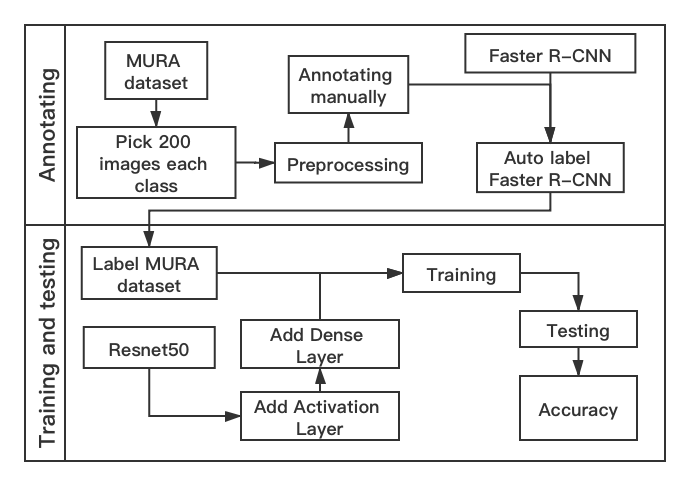
\includegraphics[width=1\columnwidth]{images/architecture.png}
\caption{Main schematic diagram: the annotation and training operations in different models.}
\end{center}
\end{figure}

The methods are improved based on the current approaches. There are two main parts showed in Figure 1.
\par On the one hand, the main process can be found in Figure 1. After reading and comparing different references, the Faster R-CNN is the best network to annotate automatically the images from MURA dataset, which has better detection accuracy and higher detection efficiency. Based on this model, firstly, small volume of training data will be labelled manually (showed in Figure 2-3), and then do the augmentation and other pre-processing operations, finally, putting data into the faster R-CNN model with transfer learning will be done. 
\begin{figure}[htbp] %  figure placement: here, top, bottom, or page
\begin{minipage}[t]{0.5\textwidth}%并排放两张图片,每张占页面的0.5,下同。
\centering
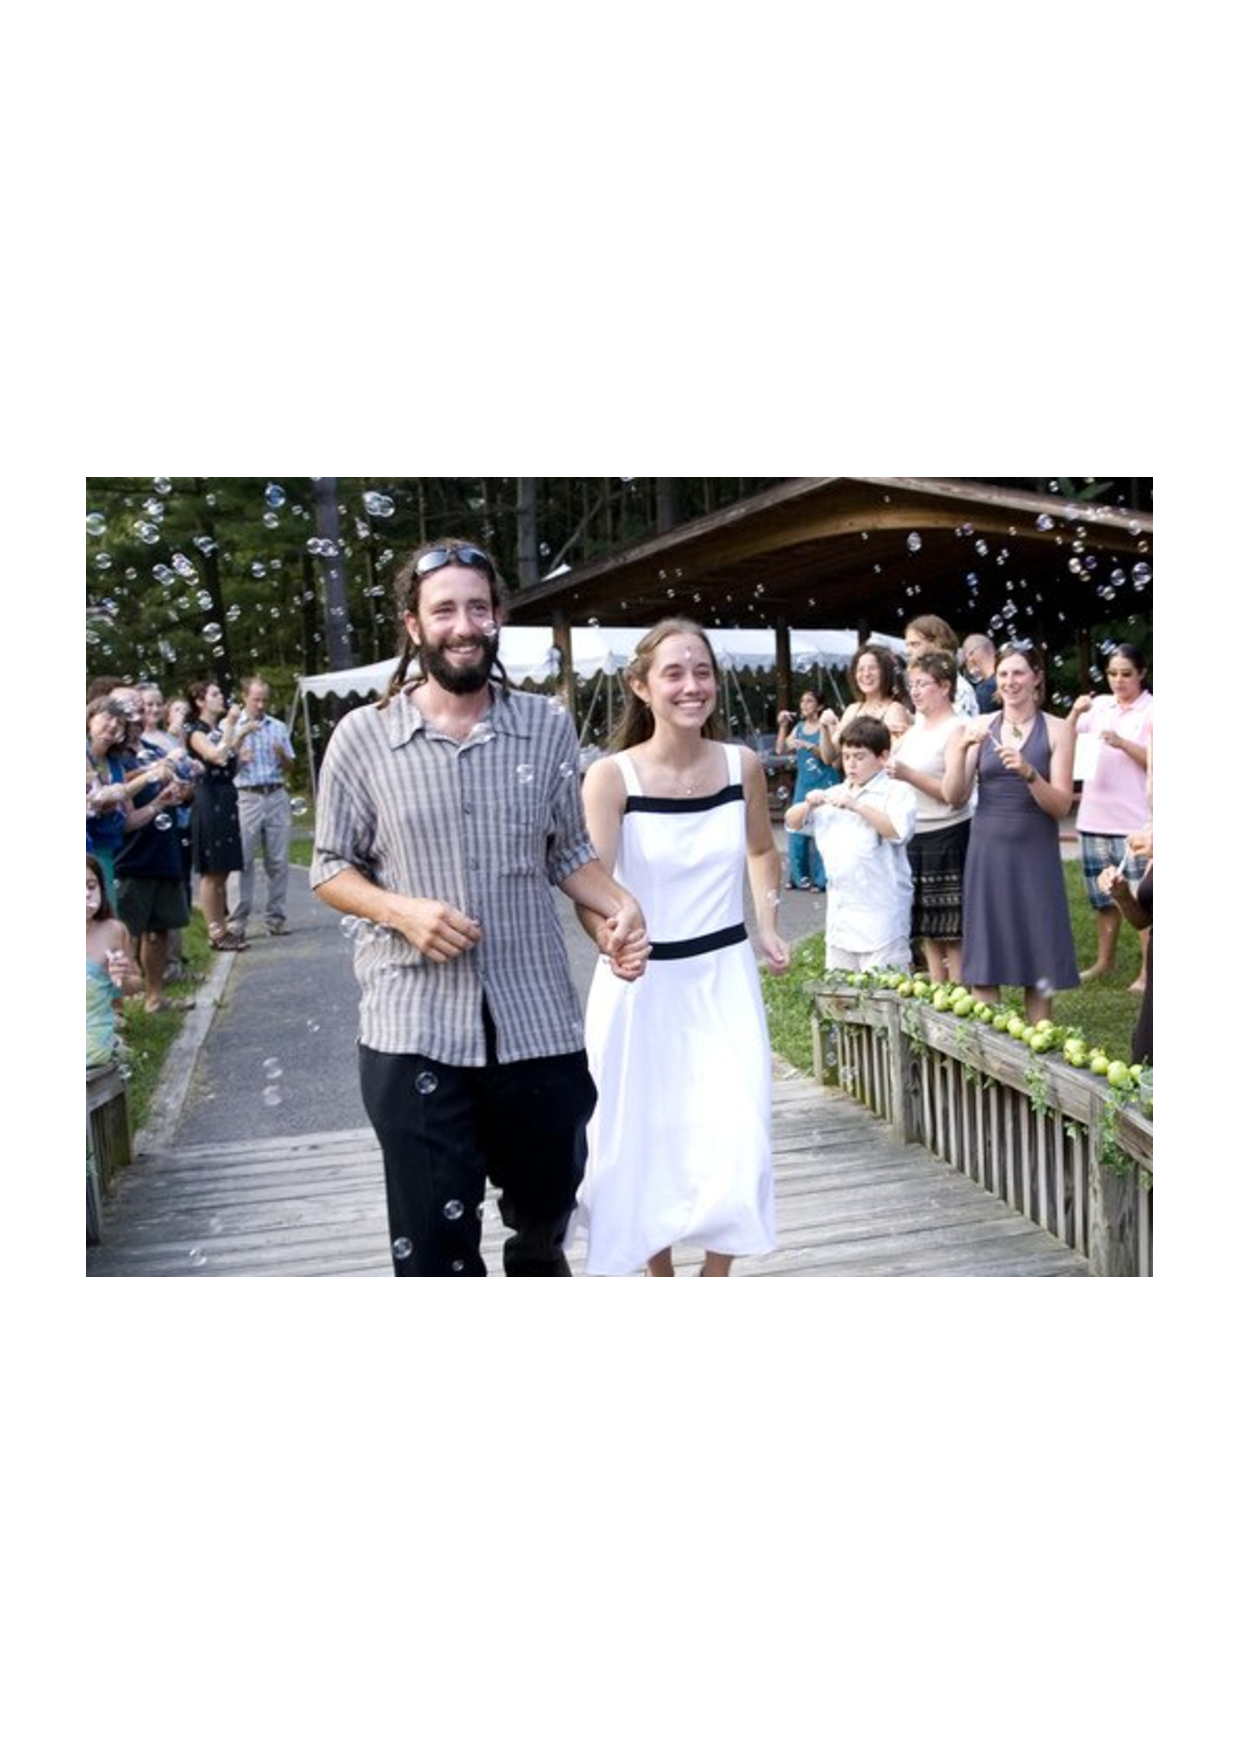
\includegraphics[width=\textwidth]{images/reference.png}
 \caption{Reference: it is the reference image with fracture.}
\end{minipage}
\begin{minipage}[t]{0.5\textwidth}
\centering
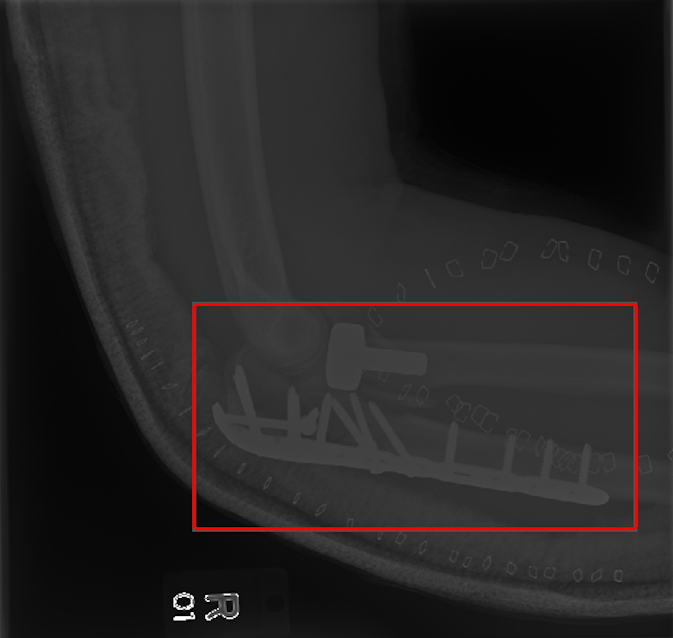
\includegraphics[width=\textwidth]{images/Annotation.png}
 \caption{Annotation: it is the annotated image after annotating the reference image.}
\end{minipage}
\end{figure}

\par On the other hand, because the various models have different accuracy and efficiency and most of them have low universality, so further work will be done by combining multiple good models. After some initial experiments, some models with great performance have been picked up from current models, which are ResNet50, Inceptions-v3 and DenseNet169. The more detailed processes based on ResNet50 are displayed in Figure As for the follow-up improvement plan, more experiments are inevitable. 



\subsection{Hardware/Software platform}
For the platform, the Google Colab with GPU and TensorFlow will be used and the Python language is the main programming language. 
\subsection{Risks and challenges}
However, there still exist amounts of challenges in this project. For example, the architecture of model is difficult to modify and adapt to the high accuracy in fracture detection, so the model should be upgraded iteratively and be tested until getting the best result from experiments. On the other hand, in order to increase the universality of model, more training images should be collected manually, such as getting them from local hospital.


\clearpage
\section{Project Plan}
From Figure 4, the detailed plan of project is displayed below. The primary task is mainly divided into some parts. Firstly, it is literature review, which is a necessary step before starting this project. Meanwhile, it includes two subtasks in the chart. Secondly, analyzing the existing methods and proposing some potential measures are very essential. And then the models will be trained by using the collected datasets. Lastly, remaining time will be used to write and revise the report and codes.

\begin{figure}
\begin{center}
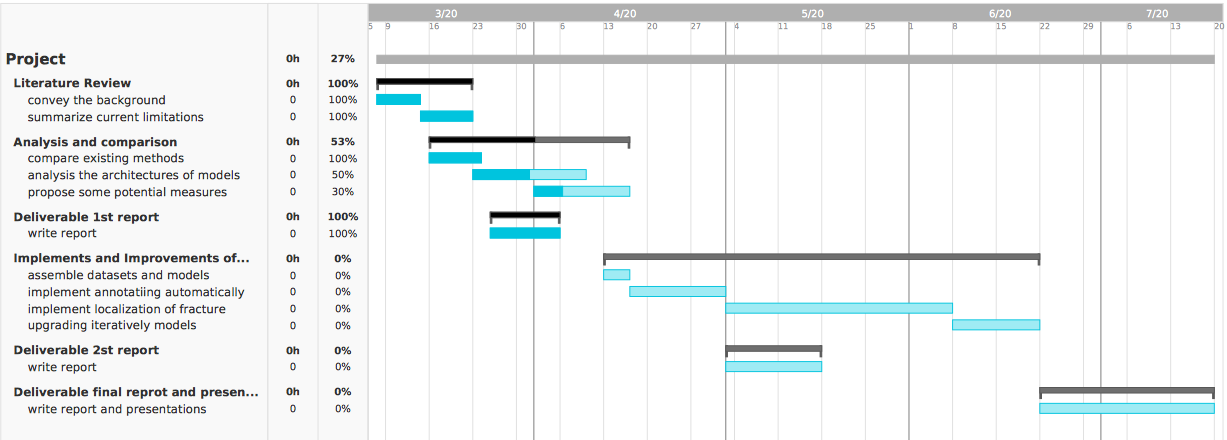
\includegraphics[width=1\columnwidth]{images/TaskGantt.png}
\caption{Project Plan: timetable in different periods}
\end{center}
\end{figure}





\clearpage
\begin{thebibliography}{99}
\bibitem{b1}Lindsey  R,  Daluiski  A,  Chopra  S,  et al  (2018).  Deep  neural  network  improves fracture  detection  by  clinicians.  Proceedings  of  the  National  Academy  of Sciences, 115(45), 11591-11596.  
\bibitem{b2} Miao, Yu Zhao, Peng-Fei Tang, Xiong-Feng Li, Yu-Qin Zhang, Li-Yuan Shi, Wei-Li Zhang, Ke Yang, Hua-Min Liu, Jian-Hua. (2019). A Method for Detecting Femur Fracture Based on SK-DenseNet. AIAM 2019: Proceedings of the 2019 International Conference on Artificial Intelligence and Advanced Manufacturing. 1-7. 10.1145/3358331.3358402. 
\bibitem{b3} Pranav Rajpurkar, Jeremy Irvin, Aarti Bagul, et al (2018). MURA: Large Dataset for Abnormality Detection in Musculoskeletal Radiographs. The Conference on Medical Imaging with Deep Learning 2018, arXiv:1712.06957v4. 
\bibitem{b4} Yahalomi, Erez Chernofsky, Michael Werman, Michael. (2019). Detection of Distal Radius Fractures Trained by a Small Set of X-Ray Images and Faster R-CNN. 10.1007/978-3-030-22871-2-69. 



\end{thebibliography}

\end{document}